\section{Hadoop Security}
\label{security}

In this section, we discuss the security vulnerabilities and also security modules of Hadoop, including arbitrary code execution, malicious user impersonation, and compromised nodes.

\subsection{Arbitrary code execution}

Users submit jobs to Hadoop in the form of MapReduce jobs, and Hadoop executes the code without inspection. Arbitrary code execution is very common in Hadoop 1.x because malicious users can submit job executing with permissions of the TaskTracker which Task Tracker is an independent Java process.

Since it is difficult to inspect MapReduce source code, the best way is to restraint the damages of arbitrary code execution. YARN container could isolate tasks and limits task privilege. It has three implementations of container executor: 1) Default Container Executor, 2)Linux Container Executor, and 3)Docker Container Executor. The current resource types in container are 1)memory: physical/virtual memory, ratio and 2) CPU: percentage, vcores.

\subsection{Malicious user impersonation}

A big security concern of Hadoop is insufficient authentication. Hadoop does not authenticate users, and does not authenticate services. Another security concern is no integrity or secrecy protection of data and messages. The default network transport is insecure and there is no encryption over message communication.

Because of these two concerns, Hadoop could allow a malicious user to impersonate other user accounts to access data or submit MapReduce jobs. This is especially common in Hadoop ecosystem (e.g., Oozie~\cite{oozie}, Hbase).

To handle the problem of malicious user impersonation, Hadoop builds two modes to differentiate security level and requirements: non-secure mode, and secure mode.

In non-secure mode, Hadoop has no authentication, end user accounts which send out communication messages with Hadoop are regarded as Hadoop user accounts by default. For example, different users on different systems with same user name are regarded as same Hadoop user.

In secure mode, Hadoop applies authentication and data confidentiality. Kerberos Security module is added, and Hadoop RPC and HTTP communication messages are encrypted. The security framework of Hadoop secure mode is shown as below.

\begin{figure}[t]
  \centering
  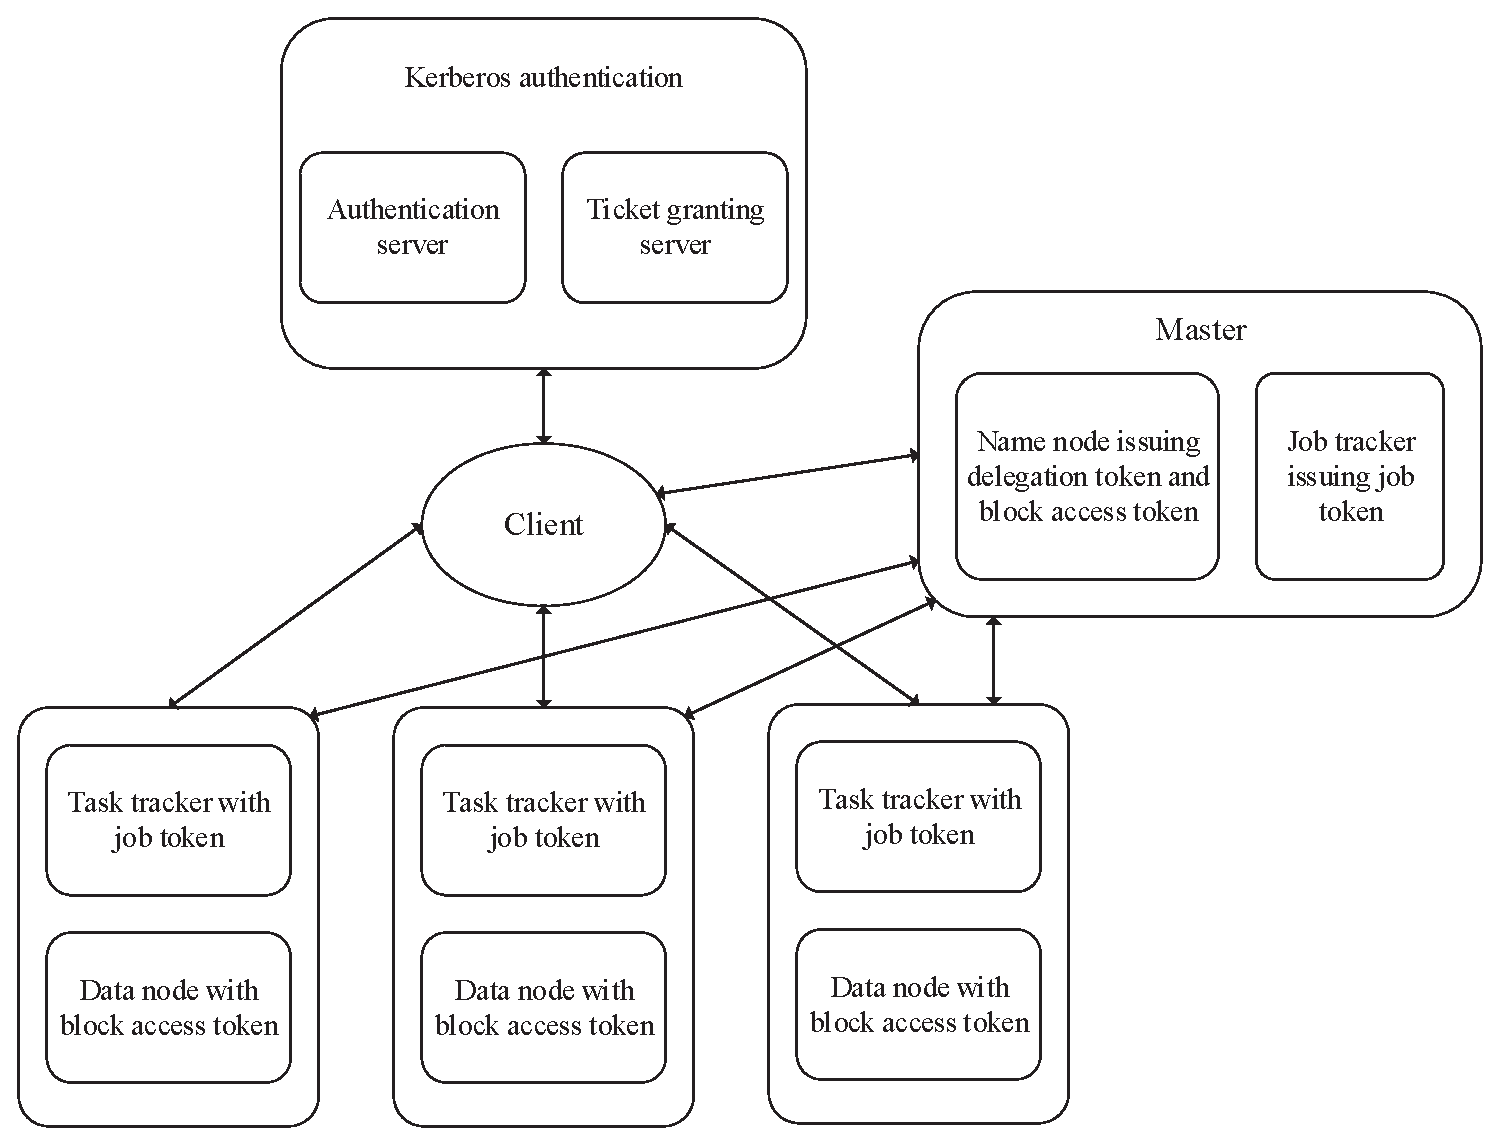
\includegraphics[width=3in]{figs/security_hadoop.eps}
  \caption{A high-level architecture of our approach}
  \label{fig:overview}
\end{figure}

As seen in the figure, kerberos authentication module has the authentication server and the ticket granting server. Tokens are used to control access to the jobs and data blocks inside HDFS.There exists three types of tokens for HDFS access namely: delegation token, block access token, and job token.

Hadoop clients use RPC which is a Hadoop’s library to access most Hadoop services. In insecure versions of Hadoop, the users login name is determined from the client OS and sent across as part of the connection setup. For authenticated clusters, all RPC’s connect using simple authentication and secure layer(SASL). Data transfer Protocol is used when reading or writing data to HDFS, by clients.

\subsection{Compromised nodes}

Compromised nodes are common in cloud system which means an attacker who has compromised just one node could introduce arbitrary errors into computations, so that the integriy of MapReduce job results could be compromised as well.

This problem is described in “Hatman:Intra-cloud Trust Management for Hadoop” in Cloud Computing , 2012.  Data and computation integrity and security are major concerns for users of cloud computing facilities. Many production-level clouds optimistically assume that all cloud nodes are equally trustworthy when dispatching jobs; jobs are dispatched based on node load, not reputation. This increases their vulnerability to attack, since compromising even one node suffices to corrupt the integrity of many distributed computations. Hatman is the first full-scale, data-centric, reputation-based trust management system for Hadoop clouds. Hatman dynamically assesses node integrity by comparing job replica outputs for consistency.

Since containers provide isolated environment, it could at some extent prevent malicious user on the compromised nodes to tamper MapReduce job results. 
